\documentclass[12pt, twoside]{article}
\usepackage[letterpaper, margin=1in, headsep=0.5in]{geometry}
\usepackage[english]{babel}
\usepackage[utf8]{inputenc}
\usepackage{amsmath}
\usepackage{amsfonts}
\usepackage{amssymb}
\usepackage{tikz}
\usetikzlibrary{quotes, angles}
\usepackage{graphicx}
\usepackage{enumitem}
\usepackage{multicol}
\usepackage{hyperref}

\newif\ifmeta
\metatrue %print standards and topics tags

\title{IB Mathematics}
\author{Chris Huson}
\date{September 2021}

\usepackage{fancyhdr}
\pagestyle{fancy}
\fancyhf{}
\renewcommand{\headrulewidth}{0pt} % disable the underline of the header
\raggedbottom


\fancyhead[LE]{\thepage}
\fancyhead[RO]{\thepage \\ Name: \hspace{4cm} \,\\}
\fancyhead[LO]{BECA / IB Math 01-Linear functions\\* 8 October 2021}

\begin{document}

\subsubsection*{Quiz: I can model with linear functions}
Equations of a straight line: $f(x)=mx+c$, $ax+by+d=0$, $(y-y_1)=m(x-x_1)$\\[0.25cm]
Gradient: $\displaystyle m=\frac{y_2-y_1}{x_2-x_1}$ \vspace{1cm}
\begin{enumerate}
\item A linear function $f$ is graphed below.
\begin{multicols}{2}
\begin{enumerate}
  \item Write down it's slope.\\ $m=$
  \vspace{0.25cm}
  \item Write down it's $y$-intercept.\\ $b=$
  \vspace{0.25cm}
  \item Write down the equation of the line.
  \vspace{1cm}
  \item State the coordinates of the point $Q$.
\end{enumerate} \vspace{.5cm}
  \begin{center} 
  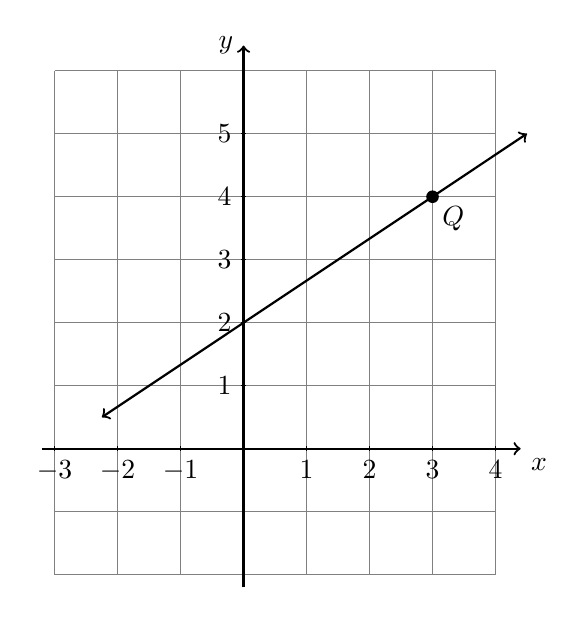
\begin{tikzpicture}[scale=0.8]
    \draw [help lines] (-3,-2) grid (4,6);
    \draw [thick, ->] (-3.2,0) -- (4.4,0) node [below right] {$x$};
    \draw [thick, ->] (0,-2.2)--(0,6.4) node [left] {$y$};
    \foreach \x in {-3,-2,-1,1,2,...,4} \draw (\x cm,1pt) -- (\x cm,-1pt) node[anchor=north] {$\x$};
    \foreach \y in {1, 2, 3, 4, 5} \draw (1pt,\y cm) -- (-1pt,\y cm) node[anchor=east] {$\y$};
    \draw [thick, <->,smooth,samples=20,domain=-2.25:4.5] plot(\x,0.667*\x+2);
    \fill (3,4) circle[radius=0.1] node[below right]{$Q$};
  \end{tikzpicture}
  \end{center}
\end{multicols}

\item Write the linear equation $y+5=2(x-4)$ in the form $y=mx+c$. \vspace{4cm}

\item A line has a gradient (slope) of $\displaystyle -\frac{2}{3}$ and passes through the point $(6, 2)$. Find the equation of the line in the form $y=mx+b$.

\newpage
\item A line goes through the points $(3,3)$ and $(6, -1)$.
\begin{enumerate}
  \begin{multicols}{2}
      \item Find the gradient of the line.
      \item Find the equation of the line in the form $y=mx+b$.\vspace{2cm}
      \begin{center}
      \begin{tikzpicture}[xscale=0.7, yscale=0.7]
        %\draw [help lines] (-3,-2) grid (4,6);
        \draw [thick, ->] (-1.2,0) -- (7.4,0) node [below right] {$x$};
        \draw [thick, ->] (0,-1.2)--(0,7.5) node [right] {$y$};
        \foreach \x in {-1, 1,2, ..., 7} \draw (\x cm,4pt) -- (\x cm,-4pt) node[anchor=north] {$\x$};
        \foreach \y in {1,2,..., 7} \draw (2pt,\y cm) -- (-2pt,\y cm) node[anchor=east] {$\y$};
        \fill (3,3) circle[radius=0.1] node[above right]{$(3,3)$};
        \fill (6,-1) circle[radius=0.1] node[below left]{$(6,-1)$};
        \draw [thick, <->,smooth,samples=20,domain=2.5:6.5] plot(\x,-1.33*\x+7);
      \end{tikzpicture}
      \end{center}
    \end{multicols}
\end{enumerate} \vspace{3cm}

\item Find the equation of the line through the points $(-2,7)$ and $(6,9)$. (in the form $y=mx+c$) %y=1/4x+7.5

  \newpage
  \item A function $f$ is shown in the table. \hfill [5]
  \begin{center}
    \begin{tabular}{|l|r|r|r|r|r|r|}
      \hline
      $x$ & -2 & 0 & 2 & 4 & 6\\ 
      \hline 
      $f(x)$ & -1 & 3 & 7 & 11 & 15\\ 
      \hline 
    \end{tabular}
  \end{center}
  \begin{enumerate}[itemsep=2.5cm]
    \item Is $f$ a linear function? Why or why not?
    \item Is $f$ a direct variation? Explain.
    \item Find the gradient of the function. \vspace{1cm}
    \item Write down the equation of $f$ in the form $y=mx+c$
    \item Complete the table of the inverse of $f$.
      \begin{center}
        \begin{tabular}{|l|r|r|r|r|r|r|}
          \hline
          $x$ & \hspace{1cm} & \hspace{1cm} & \hspace{1cm} & \hspace{1cm} & \hspace{1cm}.\\[1cm] 
          \hline 
          $f^{-1}(x)$ & \hspace{1cm} & \hspace{1cm} & \hspace{1cm} & \hspace{1cm} & \hspace{1cm}.\\[1cm] 
          \hline 
        \end{tabular}
      \end{center}
  \end{enumerate}

\newpage

\item A function $\displaystyle f(x)=\frac{3}{4}x-2$ is graphed below.
\begin{enumerate}
  \item Complete the T-table of values for the function on the left.
  \vspace{0.5cm}
  \item Write down the values for the inverse function in the right T-table.
  \vspace{0.5cm}
  \item Draw the line for the inverse function on the graph.
\end{enumerate}
  \begin{center} 
  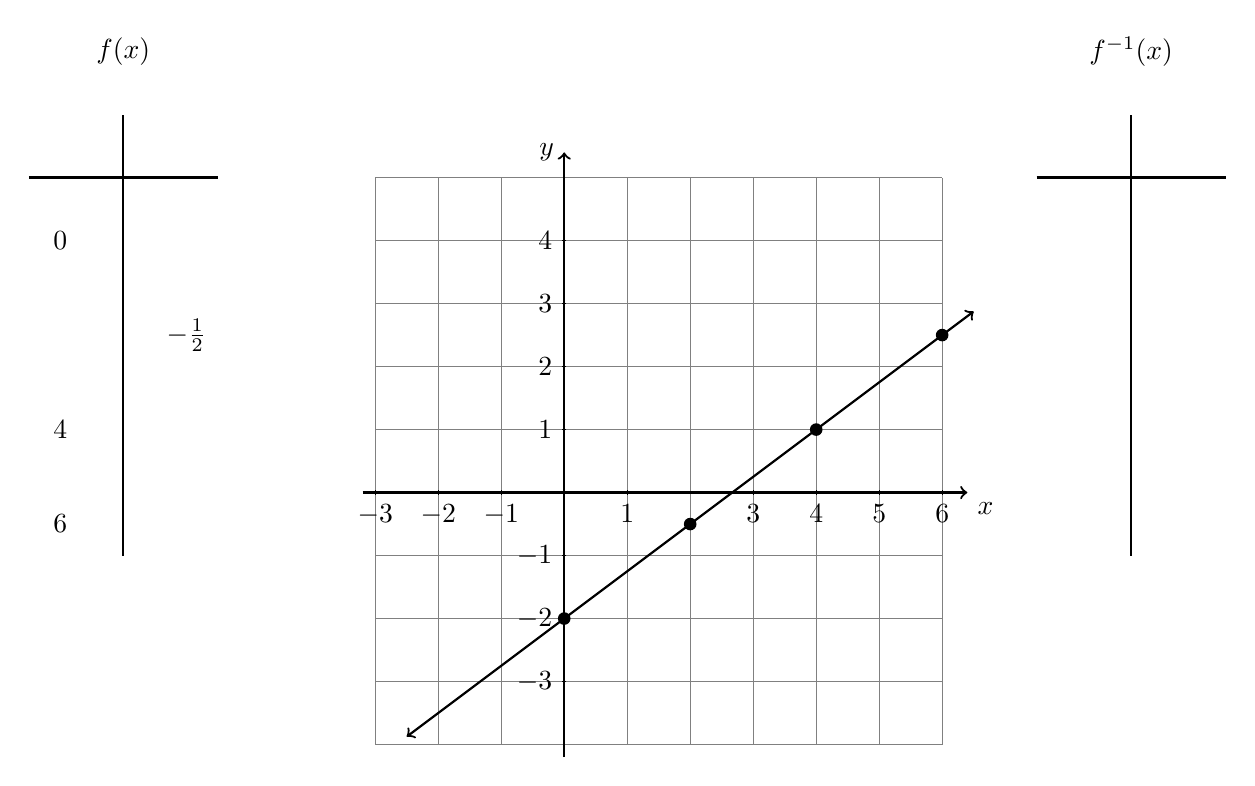
\begin{tikzpicture}[scale=0.8]
    \draw [help lines] (-3,-4) grid (6,5);
    \draw [thick, ->] (-3.2,0) -- (6.4,0) node [below right] {$x$};
    \draw [thick, ->] (0,-4.2)--(0,5.4) node [left] {$y$};
    \foreach \x in {-3,-2,-1,1,3,4,5,6} \draw (\x cm,1pt) -- (\x cm,-1pt) node[anchor=north] {$\x$};
    \foreach \y in {-3,-2,-1,1, 2, 3, 4} \draw (1pt,\y cm) -- (-1pt,\y cm) node[anchor=east] {$\y$};

    \draw [thick, <->,smooth,samples=20,domain=-2.5:6.5] plot(\x,0.75*\x-2);

    \draw [thick] (-7,-1) -- (-7,6);
    \draw [thick] (-8.5,5) -- (-5.5,5);
    \node at (-7,7){$f(x)$};
    \draw [thick] (9,-1) -- (9,6);
    \draw [thick] (7.5,5) -- (10.5,5);
    \node at (9,7){$f^{-1}(x)$};
    \node at (-8,4){$0$}; \node at (-6,2.5){$-\frac{1}{2}$}; 
    \node at (-8,1){$4$}; 
    \node at (-8,-0.5){$6$};
    \fill (0,-2) circle[radius=0.1];
    \fill (2,-0.5) circle[radius=0.1];
    \fill (4,1) circle[radius=0.1];
    \fill (6,2.5) circle[radius=0.1];
  \end{tikzpicture}
  \end{center}

\item Find the inverse function of $\displaystyle f(x)=\frac{3}{5}x-6$ using algebraic methods.

\end{enumerate}
\end{document}